\documentclass[14pt]{extreport}
\usepackage{cmap}
\usepackage[utf8]{inputenc}
\usepackage[english,ukrainian]{babel}
\usepackage{graphicx}
\usepackage{geometry}
\usepackage{listings}
\usepackage{amsmath}
\usepackage{float}
\geometry{
	a4paper,
	left=20mm,
	right=20mm,
	top=20mm,
	bottom=20mm
}
\lstset{
	language=bash,
	tabsize=4,
	breaklines,
	keepspaces,
	showstringspaces=false,
}
\graphicspath{ {./pictures} }
\setlength{\parindent}{4em}

\newcommand\subject{Конструювання програмного забезпечення}
\newcommand\lecturer{доцент кафедри ПЗ\\Сердюк П.В.}
\newcommand\teacher{доцент кафедри ПЗ\\Сердюк П.В.}
\newcommand\mygroup{ПЗ-32}
\newcommand\lab{5}
\newcommand\theme{Angular}
\newcommand\purpose{Ознайомлення з засобами розробки Angular}

\begin{document}
\begin{normalsize}
	\begin{titlepage}
		\thispagestyle{empty}
		\begin{center}
			\textbf{МІНІСТЕРСТВО ОСВІТИ І НАУКИ УКРАЇНИ\\
				НАЦІОНАЛЬНИЙ УНІВЕРСИТЕТ "ЛЬВІВСЬКА ПОЛІТЕХНІКА"}
		\end{center}
		\begin{flushright}
			Інститут \textbf{КНІТ}\\
			Кафедра \textbf{ПЗ}
		\end{flushright}
		\vspace{200pt}
		\begin{center}
			\textbf{ЗВІТ}\\
			\vspace{10pt}
			До лабораторної роботи № \lab\\
			\textbf{На тему}: “\textit{\theme}”\\
			\textbf{З дисципліни}: “\subject”
		\end{center}
		\vspace{40pt}
		\begin{flushright}
			
			\textbf{Лектор}:\\
			\lecturer\\
			\vspace{10pt}
			\textbf{Виконав}:\\
			
			студент групи \mygroup\\
			Коваленко Д.М.\\
			\vspace{10pt}
			\textbf{Прийняв}:\\
			
			\teacher\\
			
			\vspace{28pt}
			«\rule{1cm}{0.15mm}» \rule{1.5cm}{0.15mm} 2023 р.\\
			$\sum$ = \rule{1cm}{0.15mm}……………\\
			
		\end{flushright}
		\vspace{\fill}
		\begin{center}
			\textbf{Львів — 2023}
		\end{center}
	\end{titlepage}
		
	\begin{description}
		\item[Тема.] \theme.
		\item[Мета.] \purpose.
	\end{description}

	\section*{Лабораторне завдання}
	Створити проект відповідно до завдання з БД або КПЗ проектів. 
	
	\section*{Хід роботи}
	
	\begin{small}
		\begin{lstlisting}
		\end{lstlisting}
	\end{small}
	
	\begin{figure}[H]
		\centering
		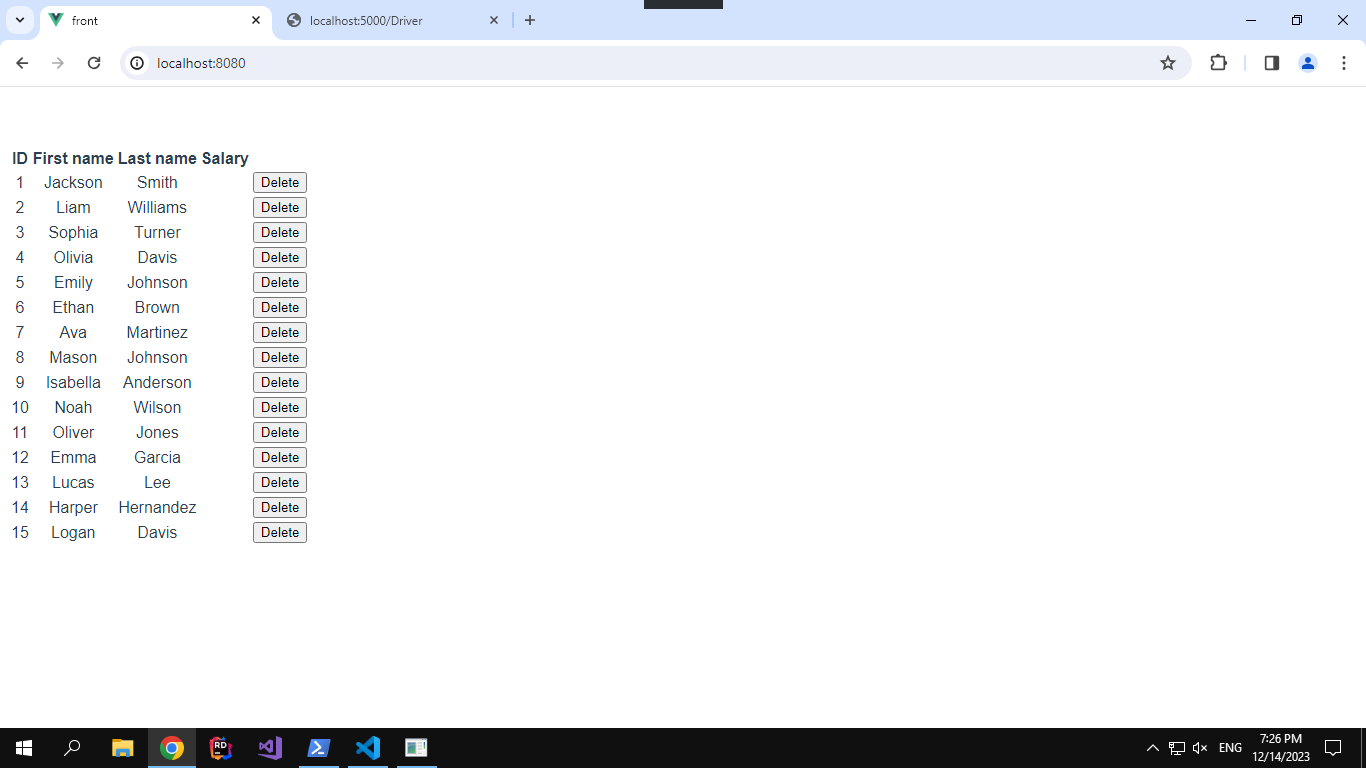
\includegraphics[scale=0.6]{1}
		\caption{Виконання програми}
	\end{figure}
	
	
	\section*{Висновок}
	Виконуючи дану лабораторну роботу я розробив додаток що виконує запити на бекенд та відображає дані за допомогою десеріалізації джсону.
	
	
	 
\end{normalsize}
\end{document}
